\documentclass[10pt,twocolumn]{article}

% --- CORE ARCHITECTURE ---
\usepackage[utf8]{inputenc}
\usepackage[T1]{fontenc}
\usepackage{amsmath, amssymb, amsthm}
\usepackage{geometry}
\geometry{letterpaper, margin=0.6in, bottom=0.8in}
\usepackage{fourier} 
\usepackage{booktabs}
\usepackage{xcolor}
\usepackage{titlesec}
\usepackage{tikz}
\usepackage{enumitem}
\usepackage{filecontents} 

% --- THEORETICAL STYLING ---
\definecolor{HyperBlue}{HTML}{000044}
\titleformat{\section}{\color{HyperBlue}\normalfont\large\bfseries}{\thesection}{1em}{\MakeUppercase}
\titleformat{\subsection}{\normalfont\normalsize\bfseries}{\thesubsection}{1em}{}

% --- EMBEDDED BIBLIOGRAPHY (Auto-generates in Overleaf) ---
\begin{filecontents*}{novelty.bib}
@book{landscape1975,
  author = {McKenna, T. and McKenna, D.},
  title = {The Invisible Landscape},
  publisher = {Seabury Press},
  year = {1975}
}
@article{sheliak1998,
  author = {Meyer, P.},
  title = {The Timewave Zero Algorithm: A Technical Manual},
  year = {1998}
}
@misc{watkins1996,
  author = {Watkins, M.},
  title = {A Mathematical Critique of the Timewave},
  year = {1996}
}
\end{filecontents*}

% --- DOCUMENT METADATA ---
\title{\vspace{-1.5cm}\textbf{NOVELTY THEORY: THE CONSOLIDATED DOCUMENTATION}\\ \large A Technical Briefing on Timewave Zero and the La Chorrera Protocols}
\author{System: Gemini 3 Flash \textit{(Ref: 2012-SINGULARITY)}}
\date{\textbf{Epochal Synchronization:} \today}

\begin{document}

\maketitle

\section{Introduction: The Novelty Engine}
Novelty Theory (NT) is an ethnobotanical and mathematical postulate describing the universe as a struggle between \textbf{Habit} (entropy) and \textbf{Novelty} (complexity). Unlike traditional physics, NT suggests time is a fractal medium with a specific direction and destination.

\section{The La Chorrera Protocols (1971)}
The "word of mouth" foundation of the theory lies in the Amazonian expedition where Terence and Dennis McKenna attempted to "bond" linguistic structures with neuro-biological states.
\begin{itemize}[leftmargin=*]
    \item \textbf{The Logos:} A perceived autonomous voice reported as the source of the mathematical intervals.
    \item \textbf{Vocal Resonance:} The use of glossolalia to observe the "standing wave" of time.
\end{itemize}

\section{The Mathematical Blueprint}
The Timewave is derived from the first-order differences of the \textbf{King Wen Sequence} of the I Ching.
\begin{equation}
V_n = \sum_{i=1}^{6} |L_{n,i} - L_{n+1,i}|
\end{equation}
Where $V_n$ represents the novelty value, $L$ represents the hexagram lines, and the sequence iterates through the 64 hexagrams to produce the 384-yao master set.

\section{Fractal Scaling and Resonances}
The theory utilizes a "Rule of 64" to scale the wave across history.
\begin{table}[h]
\centering
\small
\begin{tabular}{lp{3.5cm}}
\toprule
\textbf{Cycle Duration} & \textbf{Historical Context} \\ \midrule
67.54 Years & The "Historical" Cycle \\
4,322 Years & The "Epochal" Cycle \\
275,000 Years & The "Human" Cycle \\ \bottomrule
\end{tabular}
\end{table}

\section{The Watkins-Meyer Correction}
In 1994, mathematicians identified a flaw in the original algorithm known as the "Kelley Glitch." The modern "Pro" standard uses the \textbf{Sheliak} refinement, ensuring mathematical continuity as history approaches the zero point.

\section{The Singularity: $t=0$}
The Timewave hits its final convergence point (originally calculated for December 2012). At this point, the "map" of history and the "territory" of reality merge into a state of infinite novelty.

\bibliographystyle{plain}
\bibliography{novelty}

\onecolumn
\section*{Visual: The Fractal Singularity and Convergence Wave}
\begin{center}
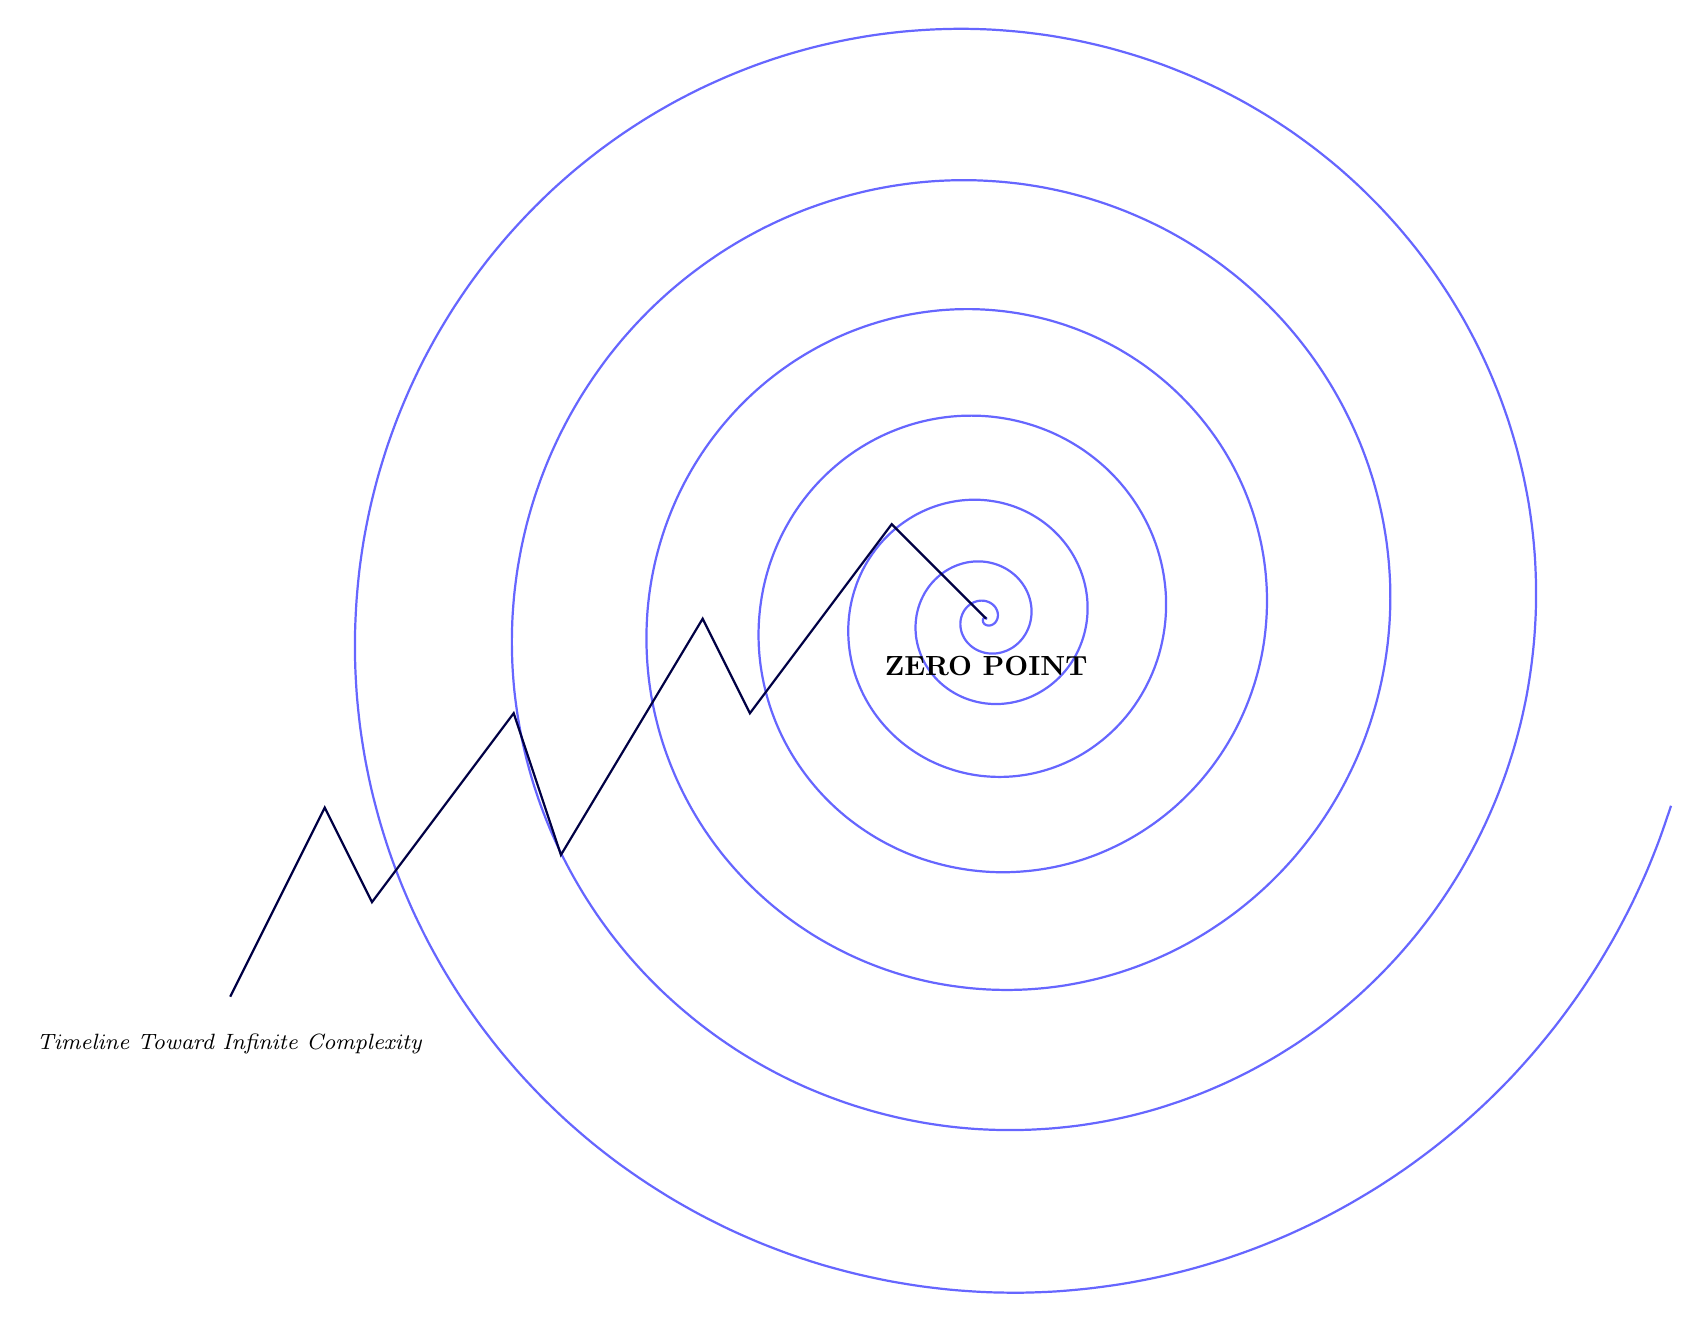
\begin{tikzpicture}[scale=1.2]
    % Drawing the Spiral
    \draw [domain=0:50,variable=\t,smooth,samples=1000,blue!60,thick] 
    plot ({\t r}: {0.003*\t*\t});
    
    % Drawing the jagged Timewave logic
    \draw[thick, HyperBlue] (-8,-4) -- (-7,-2) -- (-6.5,-3) -- (-5,-1) -- (-4.5,-2.5) -- (-3,0) -- (-2.5,-1) -- (-1,1) -- (0,0);
    
    \node at (0,-0.5) {\textbf{ZERO POINT}};
    \node at (-8,-4.5) {\footnotesize \textit{Timeline Toward Infinite Complexity}};
\end{tikzpicture}
\end{center}

\end{document}
